\chapter{Diagrammes de classes}
    Il existe deux version de diagrammes de classe pour ce projet:
    \begin{itemize}
        \item Une version schématique, réalisée lors de la conception préliminaire.
        \item Une version finale, plus complète puisque comprenant le modèle, le modèle combat, les servlet, ...
    \end{itemize}
    \section{Diagramme préliminaire}
        À cette étape de la réalisation, nous n'avions qu'un diagramme représentant le modèle dans ses grandes lignes, sans prendre en compte tout l'aspect WEB.\\
        Cet aspect a été ajouté par la suite, lors du développement.\\

        \includegraphics[scale=0.7]{graph/Classes.png}
    \section{Diagrammes préliminaire}
        Pour des questions de lisibilité, le diagramme de classe est divisé en plusieurs sous diagrammes.\\
        Pour chacun, un court descriptif expliquera le but de ce package.
        \subsection{Diagramme package Combat}
            Le package Combat modélise le combat entre un Village et une Armée.\\
            Il est en charge de la simulation d'un combat, et dépend intégralement du modèle Model.\\

            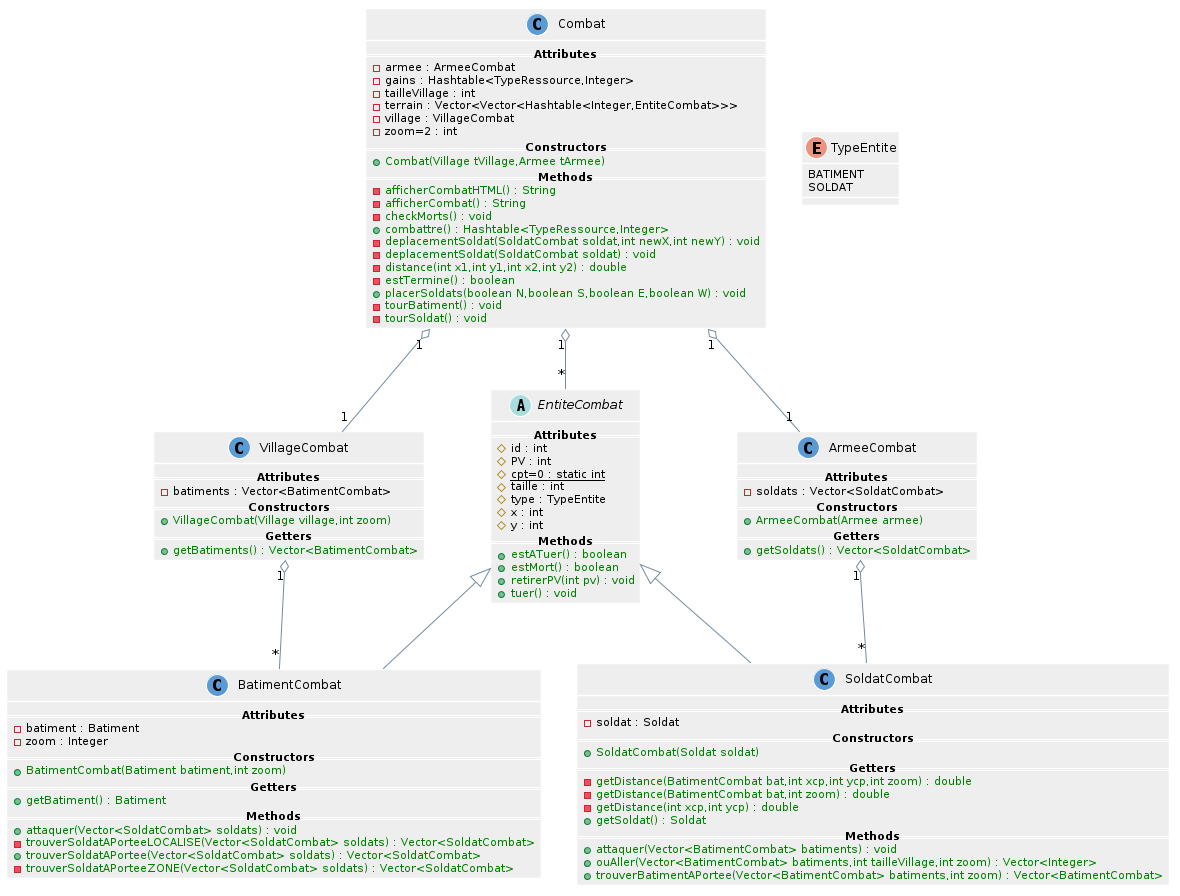
\includegraphics[scale=0.4]{ressources/images/ClassesCombat.png}
        \subsection{Diagramme package Controleur}
            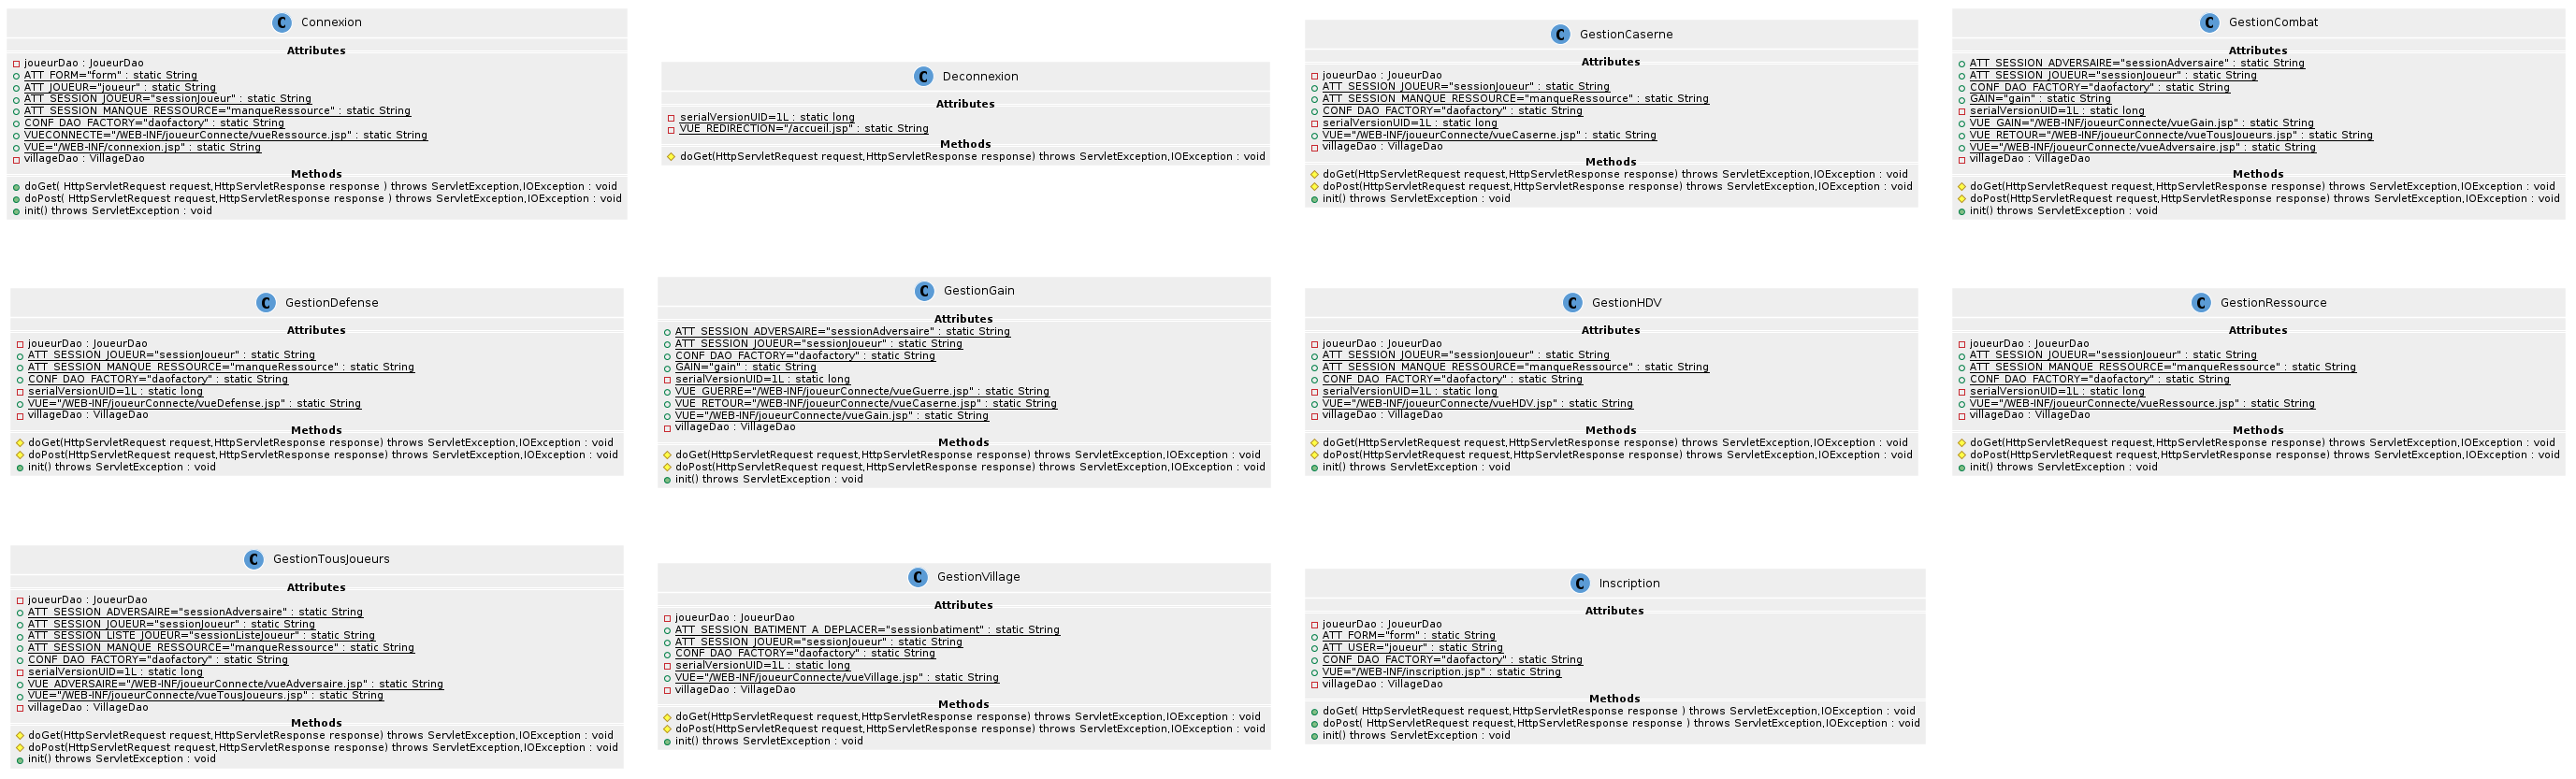
\includegraphics[scale=0.4]{ressources/images/ClassesControleur.png}
        \subsection{Diagramme package DAO}
            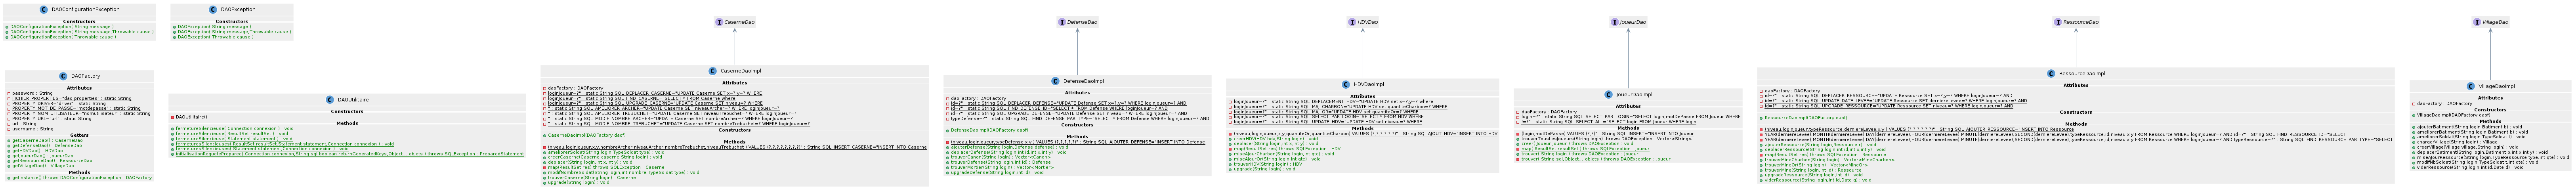
\includegraphics[scale=0.4]{ressources/images/Classesdao.png}
        \subsection{Diagramme package Model}
            Le package Model modélise l'intégralité du modèle, c'est à dire:
            \begin{itemize}
                \item L'ensemble des bâtiments.
                \item L'armée.
                \item Chacun des types de bâtiments.
                \item Chacun des types de soldats.
            \end{itemize}
            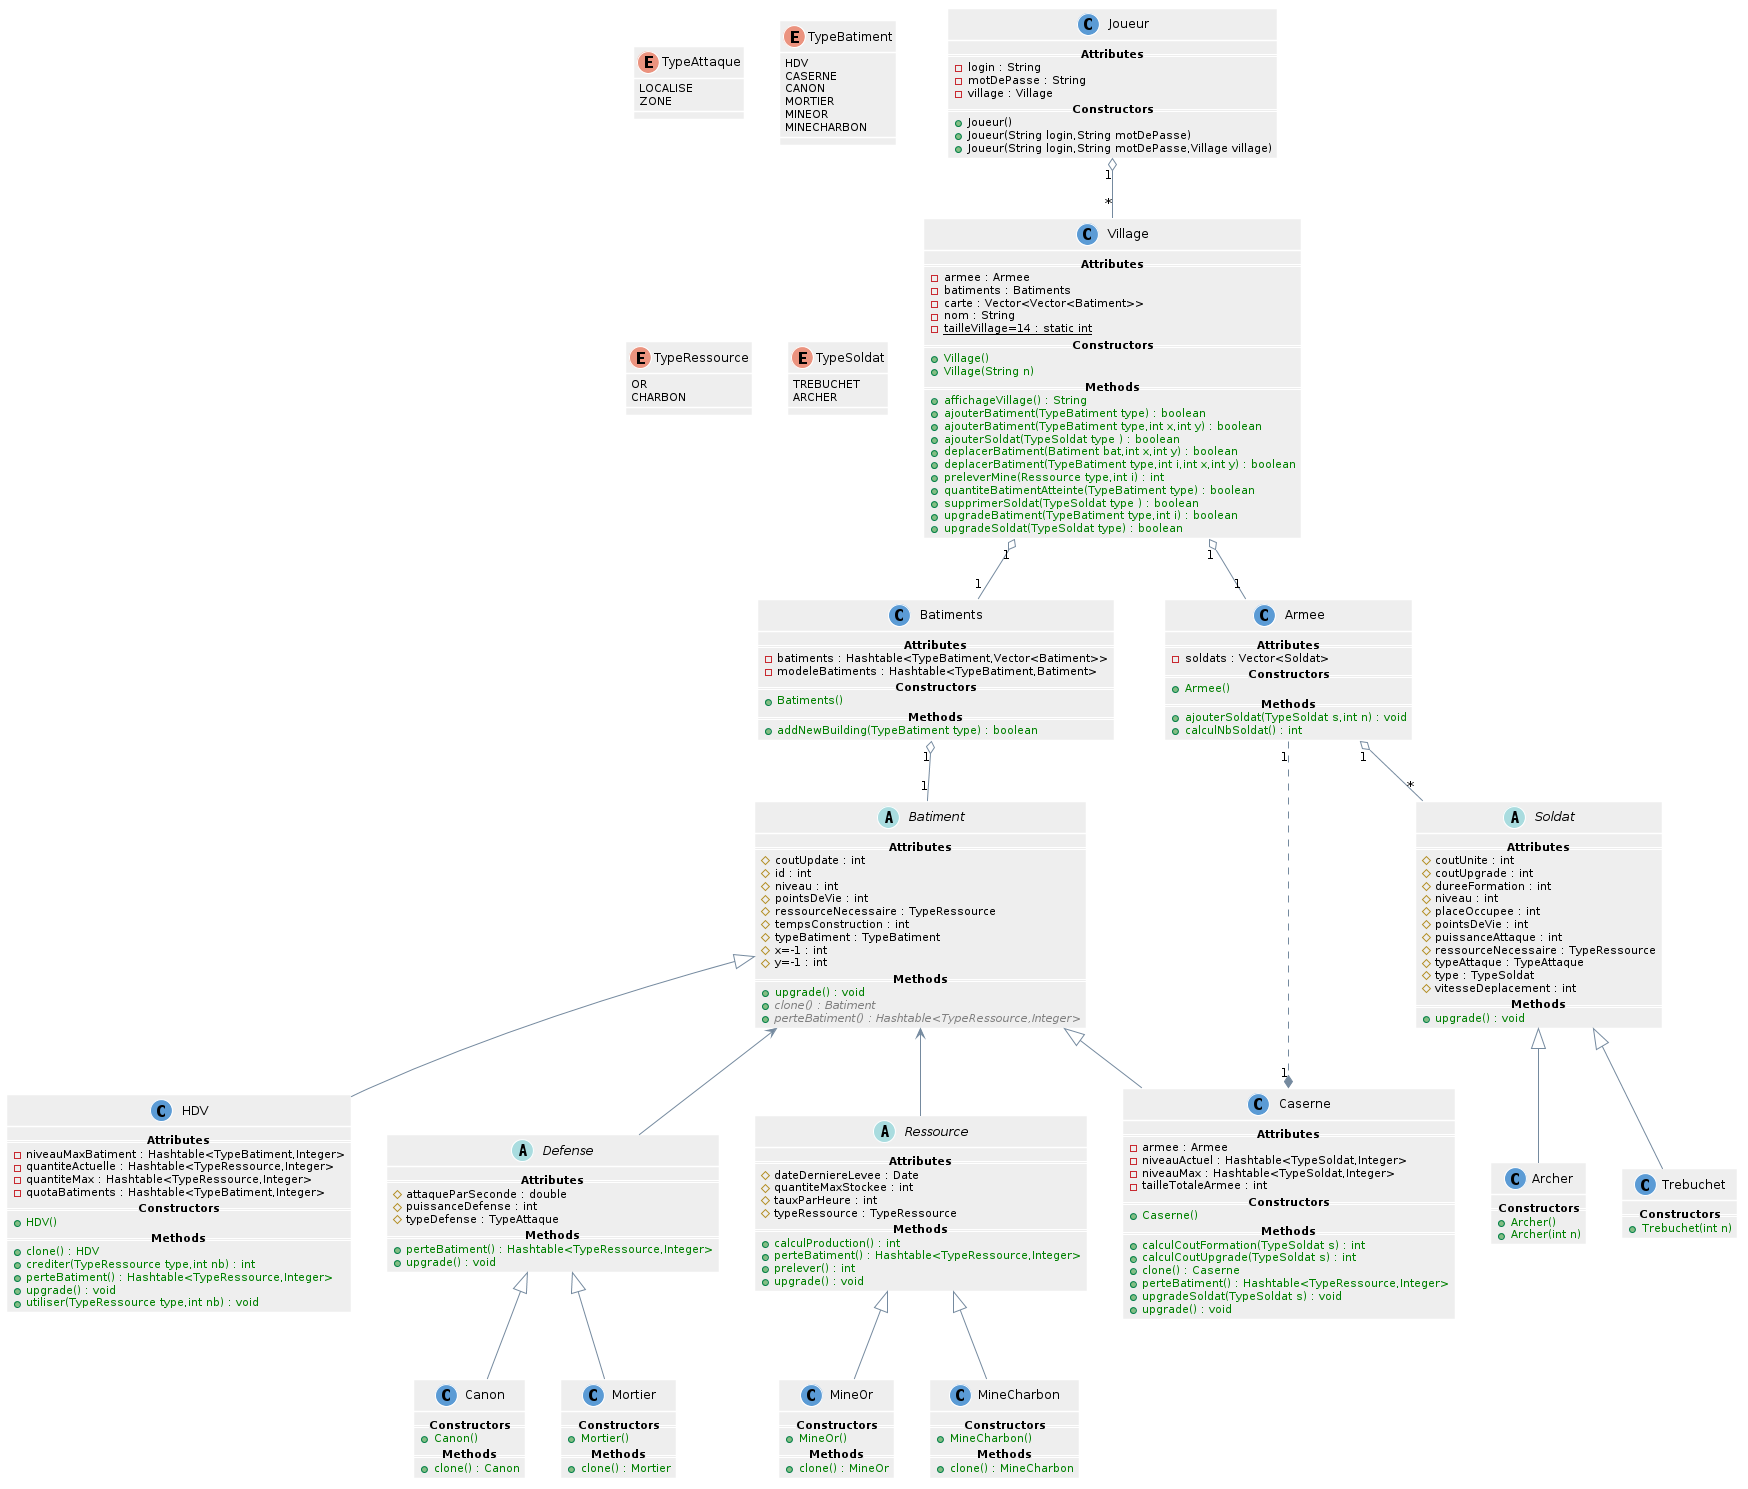
\includegraphics[scale=0.3]{ressources/images/ClassesModel.png}
